From figure \ref{fig:PNJ_climatogram} we find:
\begin{itemize}
    \item temperature lower in all scenarios: stratospheric cooling from increased CO2, most significant in summer months as expected due to higher solar irradiance
    \item wind speed in ASO higher in both SAI scenarios, consistently above 100 m/s
    \item earlier development of high winds/PNJ, about 20 m/s in june compared to both reference and control
    \item occurrence of prolonged sudden stratospheric warming events decreased, as can be inferred from the lower wind speeds and higher temperatures/greater spread at the end of the season
    \item SSW's could still occur after 2100 in the simulations in all scenarios but likely of much shorter duration, thus not showin up in monthly average values
\end{itemize}
TO DO:
\begin{itemize}
    \item extend period to 30 years
    \item add 30-60°S mean T
\end{itemize}

From figure \ref{fig:PNJ_map} we find:
\begin{itemize}
    \item higher intensity for all scenarios compared to reference
    \item lower zonal wind speed in eastern pacific, WHY? compare to EKE and absolute wind speeds? appears to be no narrowing of jet
\end{itemize}
TO DO:
\begin{itemize}
    \item add gridlines (to all maps)
    \item line of maximum at 10 hPa in same figure or additional figure?
\end{itemize}

\begin{figure}[H]
    \centering
    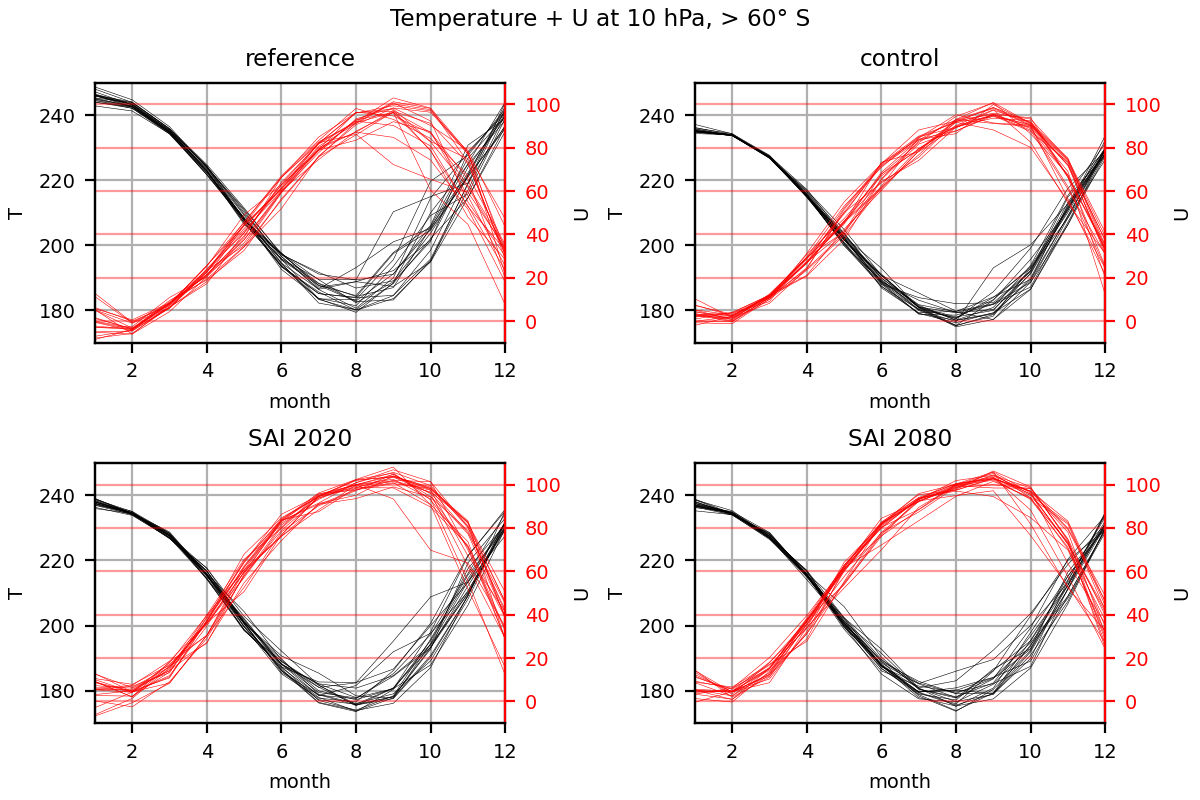
\includegraphics[width=\linewidth]{images/PNJ_climatogram.png}
    \caption{Mean temperature $>$60°S at 10 hPa in °C and zonal mean zonal wind at 60°S and 10 hPa in m/s. Shown are reference 2020-2039 and all scenarios 2111-2130}
    \label{fig:PNJ_climatogram}
\end{figure}

\begin{figure}[H]
    \centering
    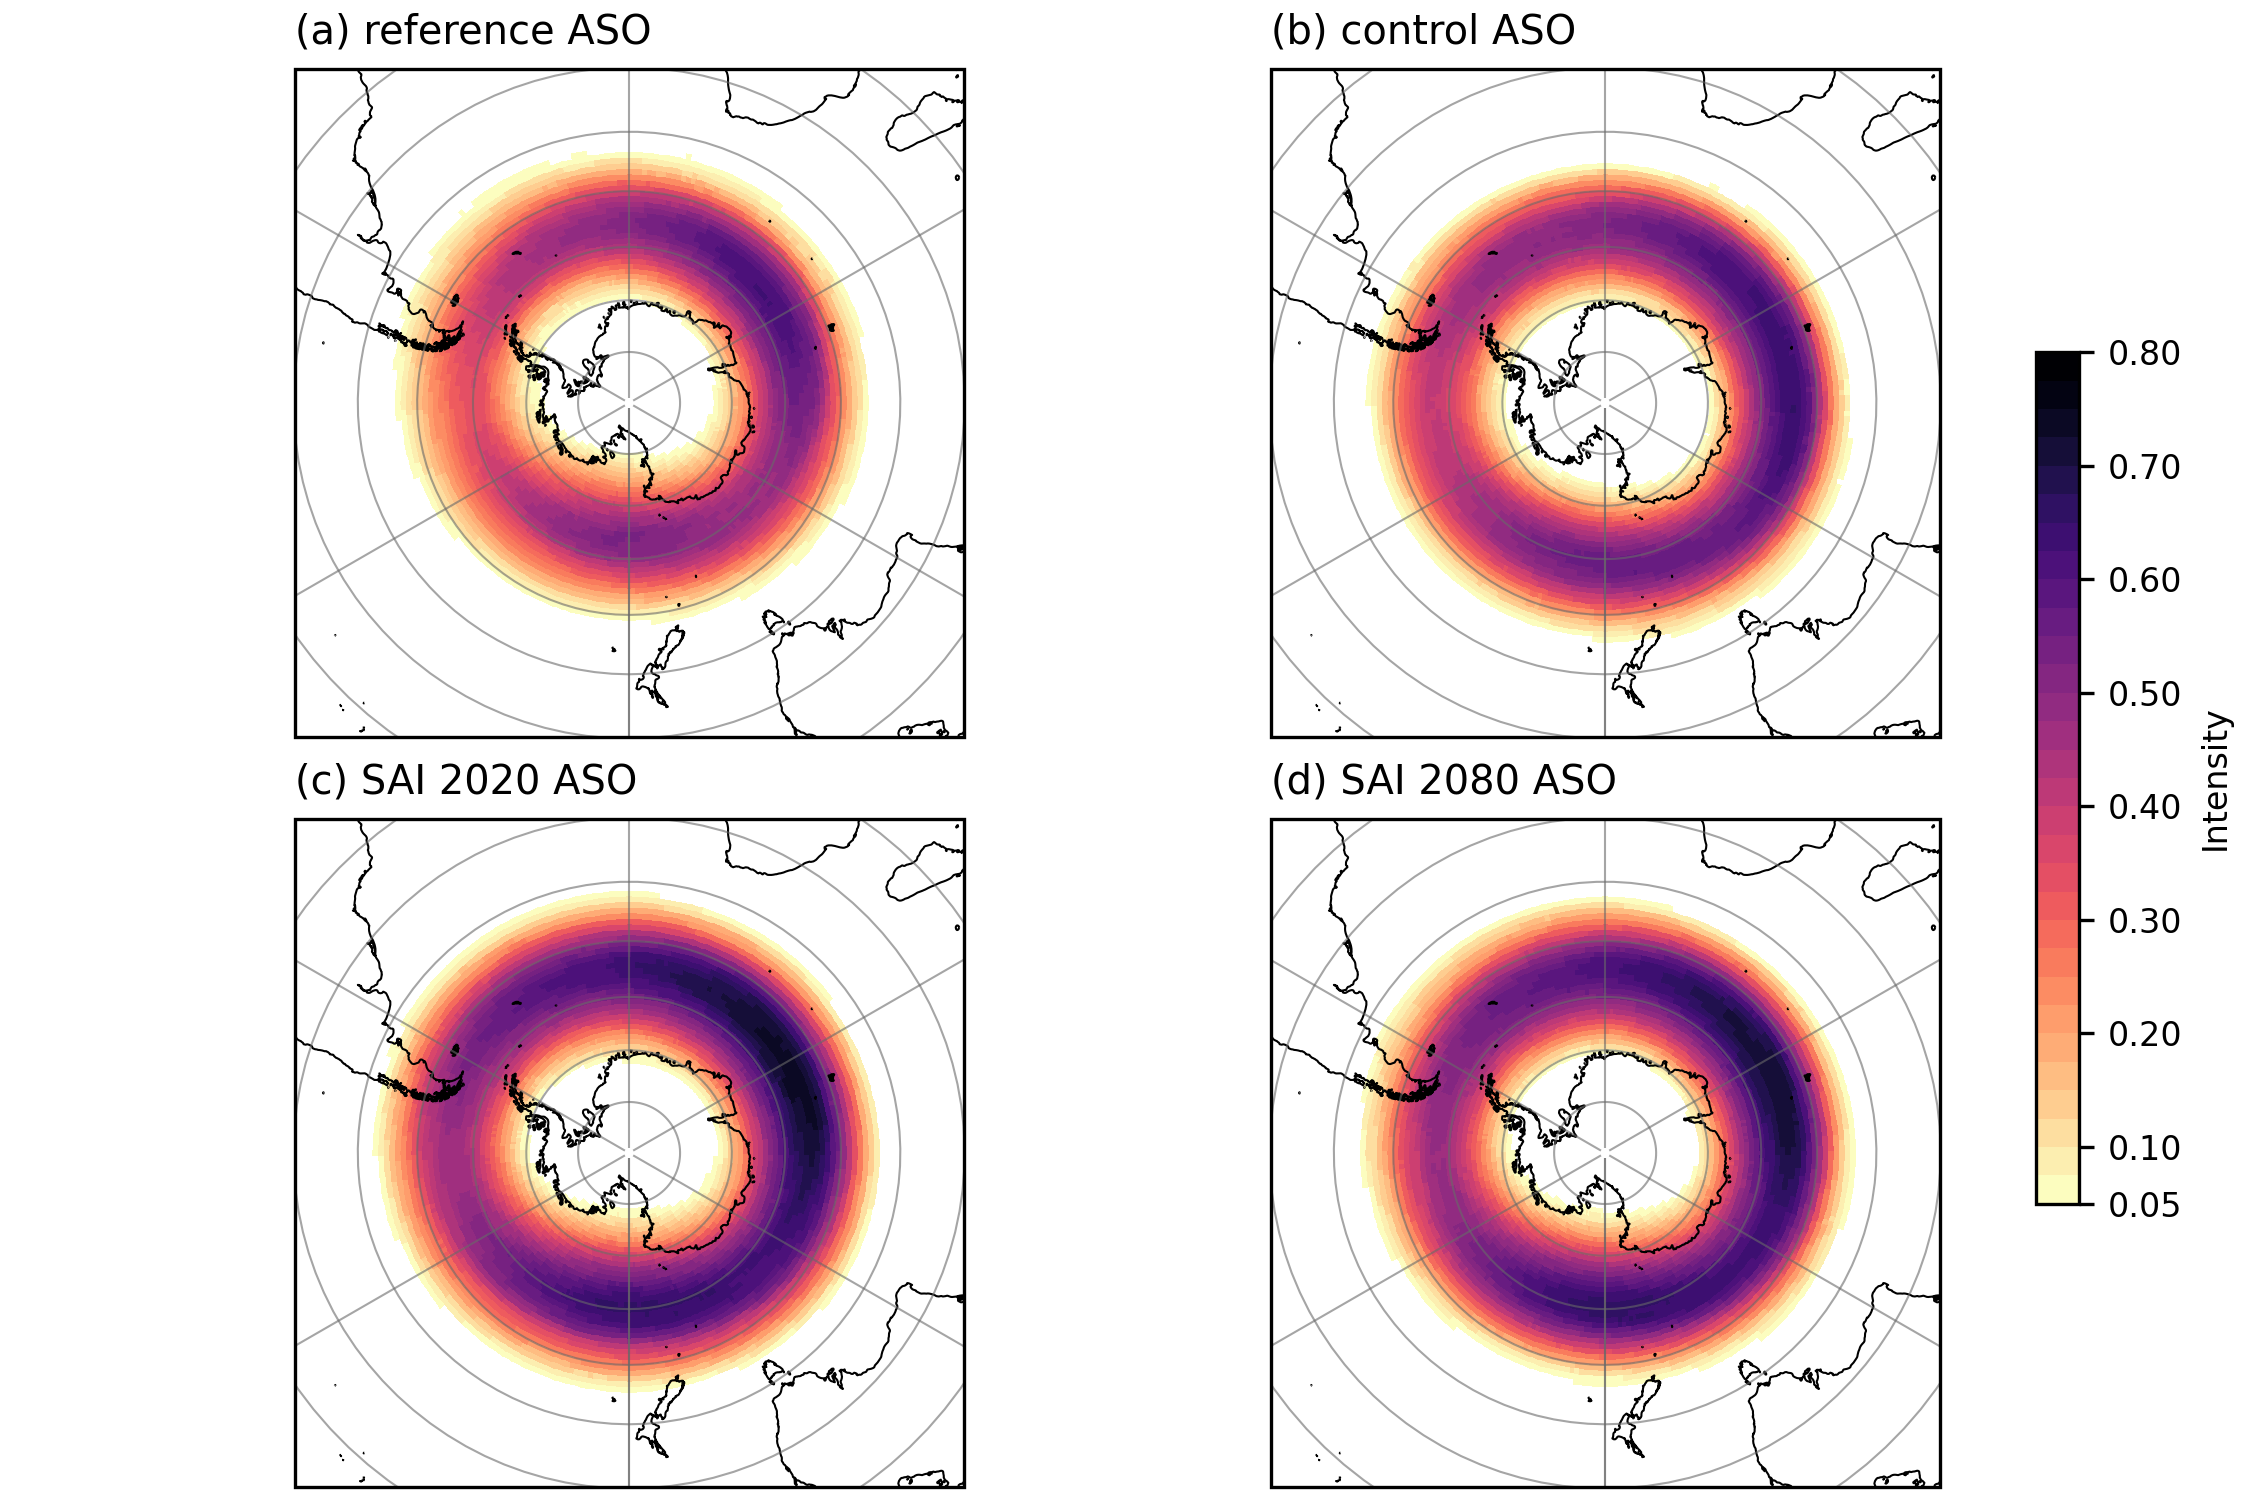
\includegraphics[width=\linewidth]{images/PNJ_map.png}
    \caption{Map of PNJ intensity above 50 hPa (?). Fractional occurence of $>$90 m/s zonal winds in each grid cell, at each model level in the months august, september and october in each time interaval. Shown are reference 2020-2039 and all scenarios 2111-2130.}
    \label{fig:PNJ_map}
\end{figure}

\begin{figure}[H]
    \centering
    
\includegraphics[width=\linewidth]{images/TREFHT_ann.eps}
    \caption{Map of PNJ intensity above 50 hPa (?). Fractional occurence of $>$90 m/s zonal winds in each grid cell, at each model level in the months august, september and october in each time interaval. Shown are reference 2020-2039 and all scenarios 2111-2130.}
    \label{fig:PNJ_map}
\end{figure}
